\chapter{Introduction}
% 1st sect: GENERAL BACKGROUND: data environments evolve. data stream processing requires being accurate efficiently.
A problem occurring in nearly every application of machine learning is the challenge of handling evolving environments, a problem known as concept drift. Meanwhile, the domain of data stream processing proposes its own set of challenges, the main one being the ability of providing accurate predictions at any time despite large volumes of data and constrained time and memory resources. The combination of these two problems, the need to adapt to evolving data while meeting the systems requirements, is complex, but common.

% there are lots of solutions to this so requirements are needed to select from them
Multitudes of approaches have been proposed as a solution to the problem of handling concept drift efficiently in stream processing systems, each with their own set of strengths. Therefore, to be able to compare the applicability of these solutions, a set of requirements should be used as a starting point. A case study is presented for this purpose, and the solution is searched for given the set of identified assumptions and requirements. 

% the context intro
The thesis at hand uses as context an on-going research project, VesselAI, aiming for applying novel machine learning to the domain of maritime. The domain in question is characteristic in the especially large volume of incoming sensor data and the slowness of vessel traffic in comparison. Additional context specifics include low-quality and heterogeneousness of data, the complexity and novelty of the deep learning models used, and the delayedness of model feedback. 

% goal
The goal of this analysis is, given the project context, to find the most optimal approach for maintaining model accuracy. In other words, from the challenges identified in the VesselAI state-of-the-art analysis \cite{D1.1}, the problem tackled is `ML model retraining is computationally very heavy: in environments where data evolves, it is urgent to use architectures that manage ML models in order to adapt to new data/tasks and retrain when necessary'. In addition to the suggested approach of lifelong learning, additional insight is gathered from the research fields of concept drift adaptation, batch learning, and AutoML.  This way literature gap of works addressing the maritime domain and automated model adaptation identified in \cite{D1.1} is addressed.   

% systems perspective
Traditionally, works addressing the problem of concept drift largely focus on how to build a model that is able to adapt to the changing environment. This thesis can, from this perspective, also be seen as a systems approach to concept drift. If a model is taken as given, it is discussed how the system organization would be able to make sure the model stays accurate. This perspective also aims to take into account the insight on best practices from the field of designing big data systems. From the lessons learned there it is especially aimed for a solution that is simple and mature enough to be applied to a real-world scenario.

% 2nd section: RESEARCH Q'S, METHODOLOGY, RESULTS SUMMARY

% outline
% main question
% exact definitions of main question
% sub-questions
% note on methodology (literature based but not systematic, non-empirical)
% results summary

% comment: the sentence on the model is a little vague, tailored means that it is made for the case not just taken from somewhere else. I'm unsure what words to mention on the model here.

% research question
The main research question addressed in this work is the following:

\begin{center}
    Given the domain context and the models used, how to organize a workflow for efficient updating of the models in order to meet the demands posed by the use case?
\end{center}

As further elaboration, by updating the model it is meant that the model parameters are changed. By efficient we mean efficiency relative to the data volume, not relative to computing resources. This means that an average high performance cluster is assumed and the target is to be able to utilise that to be able to handle as much data in as little time as possible. The domain context used is the maritime domain, and the model used is assumed to be a deep learning model operating in batch mode.

The secondary research questions considered as implications of the primary one are the following:

\begin{itemize}
    \item Is it possible to organize retraining effectively enough to handle incoming data, or does the model itself need to be adaptable?
    \item How much human intervention is required for maintaining the updating schemes; what are the possibilities of automating these workflows?
\end{itemize}

% add paragraph on results here later...

As a note on methodology, the investigation in its entirety is based on literature. Conducting a systematic literature review would be beyond the scope of this thesis, so only material directly relevant regarding the specific set of requirements is taken into account. Testing the various approaches in practice is also beyond scope; the empirical investigation of these findings is left to future works. This limits both the set of options considered to those already used in the problem domain and the evaluation to analyzig the thoroughness of existing evidence in literature.

% 3rd section: CHAPTER ROLES
% if the result is so that multiple can be good then change chap 4 description to state that the systems applying the max two best seeming options are presented.

The rest of this thesis is organized as follows:

Chapter 2 presents the necessary background knowledge to the reader: an overview of the general organization of a big data system, definitions in the field of machine learning model updating, and an introduction to the maritime domain. Chapter 3 analyzes the various model updating approaches presented previously and discusses which approaches would be most useful given the context of the case. Then, ways of automating the optimal-seeming approaches are shortly discussed. Chapter 4 synthesizes the findings above and presents an abstract overview of the system that would apply the optimal updating workflow. In addition it is discussed how certain these findings are given the quality and thoroughness of the literature used. The thesis is concluded with discussion on the applicability of the results achieved to similar problems from different domains.

\chapter[Overview on large-scale machine learning systems for maritime]{Overview on large-scale machine\\ learning systems for maritime}

% ingressi: mitä aiot rakentaa luvussa, mikä tulee esille, miksi se on tärkeää, mihin tällä kokonaisuudella pyritään

The general task of big data systems is that they should be able to handle vast amounts of data and from that be able to provide predictions in a timely manner. To position our problem of model maintenance in this larger domain, this chapter provides an introduction to the necessary background. First, the background to both deep recurrent neural networks and relevant machine learning approaches are provided. Then, the entire big data pipeline and relevant design decisions are presented on an abstract level. Lastly, the requirements of the case used to compare the maintenance approaches are derived from the application domain description.

%online learing survey has lots of definitions that can be checked!
\section[Background on neural networks and machine learning approaches for model maintenance]{Background on neural networks and machine\\ learning approaches for model maintenance}

% intro to rnn+dnn and sgd
\textbf{Neural networks} is a machine learning paradigm that takes its inspiration from the human brain. The composition of a neural network is the following. The basic building blocks are neurons, collected in a layered architecture. A single neuron composes of weights and an activation function. The neuron takes weighted signals from part of the neurons of the previous layer and determines using the activation function which weighted value it passes on neurons connected to it on the next layer. \textbf{Deep neural networks} mean networks that have more than one layer between the first and last layer. \textbf{Recurrent neural networks} are networks where there are not only connections to the next layer, but also back-connections within the same layer \cite{ben-nunDemystifyingParallelDistributed2019}. 

 Training of a deep neural network means that the weights of the neuron-to-neuron-connections are adjusted, usually using the algorithm called \textbf{stochastic gradient descent} \cite{ben-nunDemystifyingParallelDistributed2019}. Predictions to a learning task are determined by the value of the final layer after the signal has passed through the entrire network.

% approaches opening paragraph: nonestablished terminology
The terminology for machine learning approaches provided in the following section is somewhat indefinitive: as the terms for various approaches have varying interpretations in literature, their meaning cannot be definitively provided. Therefore, the following paragraphs will define how these terms are used in this work.

% problem: concept drift incl. subtypes + delayed feedback
For the problem space addressed, the central term is \textbf{concept drift}. By concept drift we mean the case where the relation between the input
data and the predicted variable change over time \cite{conceptdriftsurvey} \cite{schlimmerIncrementalLearningNoisy1986}. It is important to note that this does not mean fluctuation in data naturally occurring when sampling from a probability distribution, but when the probability distribution itself changes. As a simple example, fours repeating when throwing a dice would not be a concept drift, but changing the dice to one with multiple fours on it would characterize a drift. Concept drift can be further divided into types by the duration and scope of the drift. For duration, the terms \textbf{abrupt} and \textbf{gradual concept drift} distinguish cases where drift occurs over a short or a longer period of time \cite{zliobaiteAdaptiveTrainingSet2010}. For scope, \textbf{global} and \textbf{partial} concept drift are used to distinguish between drifts occurring in all or only in a subset of the incoming data. As a further challenge in this domain, it is common that the correct answers for the prediction tasks made by models are only available after some time \cite{delayedlabelstreams}, for which the term  \textbf{delayed feedback} will be used. 

% paradigms: what this is & is not
The terms describing machine learning approaches used for dealing with concept drifts or other changes are the following. Approaches regarding models that are capable to learn new tasks using previous training, such as a classifier being able to recognize unseen classes is called \textbf{transfer learning} \cite{iotsurvey}. \textbf{Lifelong learning} is a closely related field that explores the ability of models to adapt to new tasks, meaning new problems or environments, without losing the accuracy on previously learned tasks.  These approaches are out of the scope of this thesis. As for approaches that do not enable adjusting to new prediction tasks, \textbf{adaptive learning} refers to models able to adjust to concept drift \cite{conceptdriftsurvey}. Somewhat synonymously, \textbf{continual learning} is used to refer to models able to operate accurately over a longer period of time. Summarized, both adaptive and continual learning could be used to characterize the problem of this thesis, but only continual learning is used for the sake of clarity and as adaptive learning research primarily focuses on classifying tasks.

As for systems settings where machine learning is conducted, the follwing approaches are central. \textbf{Incremental learning} means cases where not all input data is available during training \cite{giraud-carrier_note_2000}. As a subtype of this, \textbf{online learning} refers to cases where data comes in as a stream one unit at a time, and can be processed as such or in \textbf{batches}, meaning chunks of data \cite{conceptdriftsurvey}.

% closing paragraph: what we are doing using this terminology
With the terminology presented above, our research challenge can be reformulated to be the following: The assumption is that there is a trained and validated recurrent deep neural network in production. The aim is to mitigate concept drifts using continual online learning with batch processing. 

% add here description like this: The online learning setting under consideration is one
%where data can be buffered in batches using a moving window. So we do batch mode online learning.


\section[Best practices in big data systems design: organization and principles]{Best practices in big data systems design:\\ organization and principles}
% this is a long sect... a lot of stuff like lambdakappa and edgefogcloud can be omitted if necessary, they are more so nice to knows

% intro to subsection: why this is explained.
In the following the abstract components of a data streaming system are presented to clarify which parts are to be studied in the later chapters. Best practices are presented to have general guidelines for which traits to priorize when comparing model maintaining approaches.

% list the components
% maybe add: this is an abstraction, feedback loops and multitudes of ways of implementation abstracted away
These parts in the order they operate in are: data extraction, data preparation, data storage, model training, model evaluation and validation, model registry, and model inference. It is assumed here that a ready neural network exists, as development organization concerns, however non-trivial, are out of scope of this thesis. For each of these, the main task and general design decisions to make are presented next.

\textbf{Data extraction} is responsible for handling the incoming data. Usual forms of data are either web logs, coming in from a server, or IoT data, coming in from sensors that are often geographically distant from the data ingesting component.

In big data systems data is usually coming in as a stream, constantly one record at a time. An important design decision to make here is whether the data should be processed as such or in very small chunks, called stream processing, or by collecting data into  larger chunks and processing those, called batch processing. The main advantage of using a batch representation is known to be increased throughput%(find citations here)
, while stream processing allows smaller end-to-end latencies. %(find citations here)
% the usually interpreted as stream or batch needs a ref too?

To mitigate this trade-off between throughput and latency, a popular solution is called the lambda architecture. This reference architecture has a processing unit for both batch and stream data with the stream component, so-called speed layer, handling requests for the data not yet processed by the batch layer \cite{beatingcap}. While this approach is widely accepted to solve the problem of handling highly voluminous data fast and mitigating human errors \cite{lambdakappa}, the architecture has faced criticism for being redundantly complex and forcing code duplication \cite{questioninglambda} \cite{uber} \cite{facebook}. As an alternative, the kappa architecture has been proposed, only composing of a stream processor \cite{questioninglambda}. This mitigates duplication, but retains the tradeoff with throughput and latency \cite{lambdakappa}.

\textbf{Data preparation} encompasses the processes of data cleaning, transformation, and feature engineering. Data cleaning refers to operations identifying and removing faulty data, such as values that are missing or clearly impossible. Data transformation and feature engineering are used interchangeably, both meaning processes that transform data into a format that the models used can process. A popular example in this is the mapping of plain text into word count matrices \cite{dapbook}.

While the data preparation step is often overlooked in literature,
it is a both challenging and crucial part of the system as preprocessing commonly takes up a majority of the total end-to-end latency of a machine learning system \cite{adaptivelearningsystems}. As for systems design, the most relevant decision to make is whether to clean data before it is saved to the data storage, or only when it is  needed for training. The main benefit with the first approach is that data only needs to be cleaned once, while the latter allows processing data for different models in different ways and retaining the data in its original form.
% the two approaches and their tradeoffs need a ref...

\textbf{Data storage} is used to save the data that is needed for model training. The most often used storage methods are called data warehouses and columnar databases. Here it is important to note that due to the volume of big data, storage times are generally short, usually the maximum being a few days. The other extreme is one-pass processing, which means that the processed data is not stored at all.
% data archival needs a ref.

\textbf{Model training} means tuning the model parameters in a way that it fits to the distribution of the incoming data in order to make accurate predictions from data coming in during operation.

% too short sentences, töksähtelee
The main design decision for this component regards infrastructure: distribution and parallelization. Centralized training, often run in a cloud data center, can run either on one machine or distributed across multiple cores by splitting the model or the data to parallelize the training \cite{ben-nunDemystifyingParallelDistributed2019}. As the amount of data is large, high-performance clusters and modern general processing units are used to reach required latencies \cite{iotsurvey}. The highest degree of distribution is called federated learning and refers to a setting where the training is conducted in the edge devices of a sensor network. This aims to solve the issues of moving privacy-sensitive data across the network and being able to adapt to the unique environments of each data source \cite{iotsurvey}.

\textbf{Model evaluation and validation} refers to the stage where the model is tested in various ways. For testing, usually various model metrics such as accuracy for classifiers and error statistics for regression tasks are checked \cite{iotsurvey}. These numbers can also be compared against other models, possibly models already in operation \cite{googlemlops}. Also testing different data sets and checking compatibility with the rest of the system is conducted at this stage \cite{googlemlops}.

In addition to testing, models are also optimized for the infrastructure that they are being deployed on. This can include, for example, various performance optimizations, or in case of constrained memory, model compression \cite{iotsurvey}.

\textbf{Model registry} is a centralized storage for the trained models. As trained models do not require a lot of memory, this stage has little complex design matters.

\textbf{Model inference} refers to the model being in production and answering application requests.
The most important design decision to make for this component is where to deploy the models. The options are a centralized cloud data center, the sensor network edge devices, or the so-called fog, which refers to any devices between the edge and the cloud \cite{fogsurvey}. The main advantage with the distributed approaches are, similarly to distributed training, reduced network latencies and better privacy. \cite{szeEfficientProcessingDeep2017}

The components presented above are summarized in Figure~\ref{simplepipeline}.

% the figure is too small... -> not very readable
\begin{figure}[hb]
%\begin{figure}[tbh] t= top, b = bottom, h=here
\newline
\begin{center}
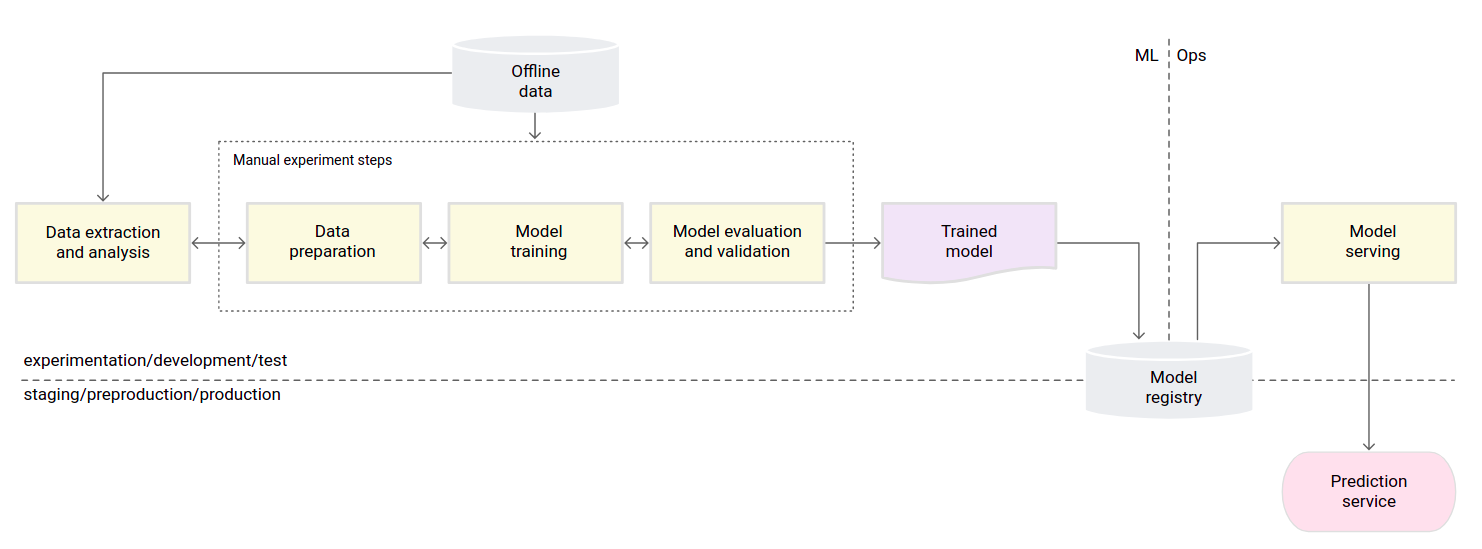
\includegraphics[width=1.0\columnwidth]{simplegoogle.png}
\caption{Abstract components of a big data analytics system. From Google Developer MLOps guide~\cite{googlemlops}.}
\label{simplepipeline}
\end{center}
\end{figure}

% model updating within inference, thesis concerns (iotsurvey has monitoring stuff if needed)
% maybe add: this is like CI and CD but CT=continuous training (from \cite{googlemlops})
The concerns of this study are within the step of model inference. This step requires, due to the evolving nature of data, a scheme for maintaining the accuracy of the model. For this purpose, a retraining pipeline, model monitoring system, and a retraining trigger need to be in place. From these parts, especially the retraining, monitoring, and trigger components are investigated. This general abstraction of the updating scheme, highlighted with the focuses of this thesis, are presented in Figure~\ref{triggerpipeline}.

% best practices + automation: mlops and automl
Lastly, the principles known to be the most important in building a successfully operating big data system are the following. These are combined lessons learned from the most mature big data systems of our time, Google MillWheel \cite{millwheel}, Facebook \cite{facebook}, Twitter storm \cite{storm@twitter} and the Uber system \cite{uber}. As the most important was deemed ease of using and improving the system, which includes modularity and simplicity. The two other principles named important across these systems were scalability and resiliency, meaning tolerance to failures and exceptions. 

As an important part of a system being easy to use was named the fact that human intervention should be minimized. This is a general trend in big data systems, as in other fields of technology. The field of MLOps aims to, similarly to DevOps, unify machine learning system development and operation, which means that automation and monitoring is advocated \cite{googlemlops}. Automation and minimizing human intervention is the topic of study in the field of \textbf{AutoML} \cite{celikAdaptationStrategiesAutomated2021}. These fields are studied for solutions promoting automation and ultimately ease of use.

% the figure is too small... -> not very readable
\begin{figure}[ht]
%\begin{figure}[tbh] t= top, b = bottom, h=here
\ \newline
\begin{center}
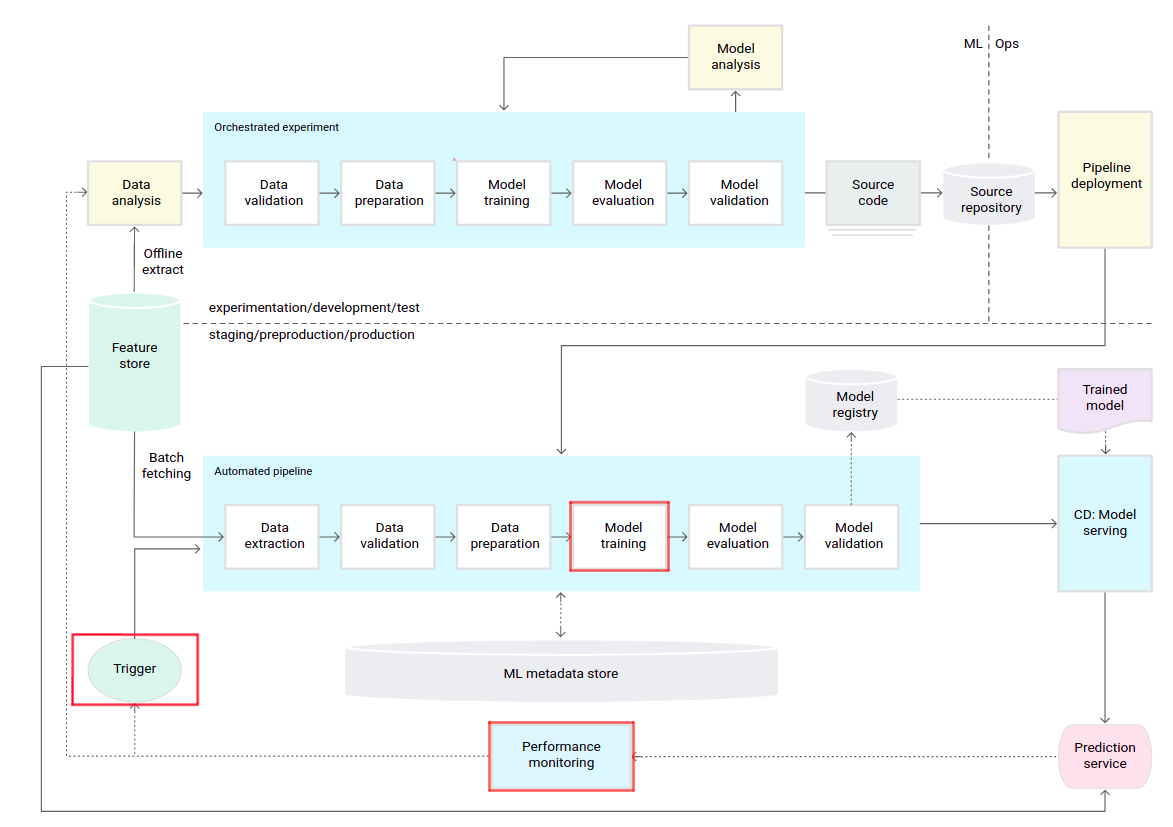
\includegraphics[width=1.0\columnwidth]{triggergooglemarked.png}
\caption{Automated retraining workflow, highlights added by the author. From Google Developer MLOps guide~\cite{googlemlops}.}
\label{triggerpipeline}
\end{center}
\end{figure}

% section conclusion: what was said & how it relates to whats to come
The principles of simplicity, scalability, resiliency and degree of automation will be another point considered when choosing the most appropriate model updating workflow: from the promising-seeming options encountered, the goal is to find one that would meet these best practices as well as possible. From the full systems perspective, this goal means handling one part of the process, model updating, as successfully as possible. Seen this way, our goal really is the means to the ends of setting up a full, efficient data processing pipeline.

\section[Context and requirements from the maritime domain]{Context and requirements from the maritime\\ domain}

% why this section: we need to know the context to know the requirements to choose the right approach 
Lastly for the background, this section introduces the maritime domain and elaborates its specialities that are then used to find the most optimal model maintenance workflow.

% maritime is global
The domain of application, maritime, differs in a few ways from others from the point or view of a sensor-based machine learning system. The most obvious difference is its global nature: while other spatial domains such as smart cities also have to take geographical distribution into account, maritime is special as it encompasses all of what the earths' surface mostly is covered by: the seas. 
% maritime is extreme heterogeneous data

As another characteristic, equally to the area that is operated in, the amount of traffic is large, which results to data volumes exceeding even what is conventionally noted as big data. Due to international regulation vessels have to send update signals of their status from every few minutes to every two seconds, depending on their speed and course \cite{maritimeinformatics}. With approximately 100, 000 ships sailing the world oceans daily \cite{maritimeinformatics}, this leads to several billion messages sent each day. To this exceptional amount of data we refer to as \textit{extreme-scale data} in this work. In addition to this, in order to provide valid maritime intelligence, other types of data such as geographical information and weather reports are needed \cite{D1.1}. Therefore, the data is not only highly voluminous, but also heterogeneous, coming in both static and dynamic forms at different velocities.

% lack of speed in terms of vessels
Added to scale, another specific of this context is speed, or more specifically, the lack of it. Depending on the size and type of the vessel, it takes from minutes to up to an hour to change course. This means that for machine learning services in this domain the acceptable end-to-end latencies are measured in seconds, even minutes. This differs greatly from other sensor system applications, where latencies are usually measured in the order of hundreds of milliseconds (e.g. \cite{anomalysystem}, \cite{facebook}, \cite{edgelatency}). This means that striving for instant response times is redundant, even of detriment, as prioritizing latency inevitably would introduce the need to make compromises in other respects, such as prediction accuracy.

% AIS intro
The main data source, the status signal data sent by vessels, called \textit{automatic identification system} (AIS) data, also has its specialities. AIS is a form of sensor data and has two types: static messages containing information such as name, destination and ship characteristics, and dynamic messages with information on the vessels' location, speed, heading, and rate of turn. The challenge with AIS data is both its highly fluctuating reporting intervals and especially its unreliability.  Things such as manually written destinations, faulty timestamping, lack of universal identifiers, misreported locations, and even illegal traffic camouflaging their operations, make identifying and correcting erroneous data both difficult and computationally expensive. In addition to faults in the data itself, another layer of error is added by the traffic system: factors such as busy areas where part of messages go lost because of overloaded receivers and vessels shutting off transmitters in fear of smugglers bring additional entropy to the data \cite{maritimeinformatics}.

% pilots
The goal of the project studied, called VesselAI, is to provide the following four pilot services to users: route forecasting for traffic monitoring and management, design of optimal ship energy systems, operating autonomous ships in short sea transport, and weather-optimized routing for long-distance voyages. In addition to this, the more abstract goals are to find a system that is suitable for both managing extreme-scale data and enabling the models to run in production over extended periods of time. The goal is also to be able to fully utilize the most modern high performance computing infrastructures in an optimal way, and develop new machine learning methods \cite{D1.1}.

% requirements derived from above
With this context and goal specification in mind, the following system goals and challenges can be stated. The general goal is to be able to provide accurate predictions not in an instant, but still in a time-constrained manner. Two main challenges arise from the combination of context and required services that most pressingly need to be addressed to reach this goal. Firstly, the nature of data used sets high demands on the training part of the workflow: storage, preprocessing, and training. Secondly, given the environment of operation, concept drift identification poses a challenge. As data quality is low, distinguishing drift from noise is hard, especially as it can be expected that the drifts will be more of the gradual type; abrupt drifts will likely be encountered only within subsets of the data. The time spans of vessel operating mean that the prediction correctness is known only after days, which means that the problem of delayed labels is very present in the domain.

How to deal with these challenges, in order to build a system able to meet its requirements, is the primary topic of inspection in the following chapters.

%outline:
% 1st paragraph: maritime specifics: geo distr, volume, vessel slowness
% 2nd paragraph: data is heterogeneous and error-prone
% missing data due to lots of traffic -> receivers dont take in everything. senders turned off bc smuggling

% 3rd paragraph: pilots n abstract aims
% the project
%	the pilots I-V: what each one aims for
%		these ml problems are difficult
%	abstract aims
%		deal with extreme scale data
%		facilitate continuous learning
%		utilize modern HPC

%data thoughts
%		static and dynamic, fast and slow paced
%			examples: map data, weather data, sensor data
%	many models only need a small fraction of the data


% combine these: the requirements.
% we want accurate solutions to hard problems not instantly, but it should not take forever either
% security is no obstacle
% obstacles to reach this
% there's a big need for data preprocessing (emphasis on workflow efficiency)
% concept drift is gradual large scale abrupt only in subset of data (napa example: vessels start anchoring somewhere)
% concept drift: noise vs drift is hard to distinguish bc error data
% correct labels to data come delayed, talking about days to couple weeks. hard to get labels also is possible. mention delayed labels


\chapter{Analysis of model updating approaches for batch learning}

% one possibility of a subsection divide here: efficient retraining, drift detestion: retraining timeliness, and mitigating the need to re-train: adaptive and lifelong learning

In this chapter, the existing solutions to the problem of efficiently updating the models are analyzed. Specifically, we assume that there is a batch-trained neural network in production, and the environment faces occasionally concept drifts, mainly of gobal and gradual, or abrupt and partial type.

There are two approaches to go about when trying to reach the goal of efficient updates outside of using adaptable models. One is to reduce the need for retraining by timing updates correctly using concept drift detection. The other is to try to make retraining as effective as possible using batch learning systems literature. As a further point on how to improve the updating scheme, the first automl solutions on the topic are presented.

% say what was chosen for presenting what was not. training set sampling is one existing approach but is not considered as it focuses predominantly on classification and there is not much material on its applicability to other tasks (double check this statement from indre thesis)

\section{Timeliness of re-training: concept drift detection}

% INAPPLICABLE SOLUTIONS: INCREMENTAL LEARNING & ENSEMBLES (CLASSIFICATION ONLY)
%in adaptive learning / concept drift adaptation the solutions have the machine learning problem quite intertwined with the adaptation mechanism \cite{celik_adaptation_2021}, and the task is dominantly a classifying task. Therefore, it is unlikely to find applicable solutions there. If those methods should be further investigated, ensembles (set of models not one model) and training set manipulation are likely to be more successful: they are popular so they are mature, and they are better for gradual-type drifts. \cite{zliobaite_driftsurvey}. worse are incremental approaches, and drift detection methods.
%ensembles better also in  \cite{mlforstreamingsurvey}:
%a mature approach for the problem

%ensemble is popular and efficient

%incremental ('feed more data') or retrain from scratch: which one is better depends very much on the data and the choice affects performance a lot \cite{celik_adaptation_2021}. this needs to be tested with ais

% TRAINING SET MANIPULATION
%data window comparisons

%- old data needs to be stored and takes up lots of memory \cite{conceptdriftsurvey} -> not applicable?

%sliding windows are popular \cite{celik_adaptation_2021}. intuitively seem useful... \cite{maritimeinformatics} (maybe) stated that removing unnecessary trajectory points makes training more efficient without degrading accuracy?

% ACTUAL DRIFT DETECTION TEXT STARTIN HERE; CAN BE EXPANDED
Concerning the implicit detection of concept drifts, the expectation of either gradual or abrupt partial drifts being present in our case is important. Additionally, abrupt drifts can be expected to be locally concentrated: an abrupt change is more likely to occur in a location than, for instance, in a feature of all sensor data. Another general point is that concept drift detection is overall better suitable for adaptation to abrupt drift as gradual drifts are hard to be distinguished from noise \cite{zliobaiteLearningConceptDrift2010}. 

Roughly, drift detectors can be divided into three classes: statistical methods triggering drifts based on perceived data distribution change, windowing techniques that compare two windows and trigger change if they differ sufficiently, and model feedback based methods that mark deteriorating model performance as drift occurring \cite{faithfullUnsupervisedChangeDetection2018}. Considering the nature of the case studied, it is necessary to detect the abrupt drifts: in cases where traffic in an area suddenly changes, for instance when a common route is shut for some reason, the performance of navigational services would deteriorate crucially unless the models are quickly updated. Additionally, due to the locality of abrupt drifts and the fact that one area represents a very small fraction of the globe, these drifts would be hard to detect unless the detection is conducted geographically distributed. Due to these specifications statistical tests seem most useful: as drift adaptation needs to be fast, model feedback based solutions work too slowly. As the memory resources in an edge device are limited, windowing might be too heavy in terms of space requirements. Which statistical test should be applied is very case dependent \cite{faithfullUnsupervisedChangeDetection2018}, so benchmarking on the data used is needed to determine the right statistic and change triggering threshold values. Thorough surveys on the possible methods and their evaluation are presented in \cite{conceptdriftsurvey} and \cite{faithfullUnsupervisedChangeDetection2018}.

As for detecting the global gradual drifts, they are expected to occur so slowly that statistical tests or windowing would be unlikely to notice them. Model performance metrics could be used, but the best-deemed of those \cite{celikAdaptationStrategiesAutomated2021} \cite{madridAutoMLPresenceDrift2019}, the DDM \cite{gamaLearningDriftDetection2004} and its improvements EDDM \cite{baena-garciaEarlyDriftDetection2006} and FHDDM \cite{pesaranghaderFastHoeffdingDrift2016}, are only applied for classification tasks. For these reasons explicit drift detection on the global level would be unlikely to add value to the updating workflow. 

% maybe add: statistical tests are an indirect indication, whereas feedback is a direct indication. therefore monitoring model feedback should also be in place because that would then notice faults in the drift detector: does model accuracy correlate with the detected drifts or not?

\section{Optimizing re-training: batch learning}

the question here is a more general one: how to train efficiently

Recurrent neural networks can be either trained from scratch or fed with new data as such, model does not need to be 're-feeding' capable

\cite{szeEfficientProcessingDeep2017} \cite{jia_highly_2018} \cite{de_sa_high-accuracy_2018}: 
states that dnn training can take hours to days. This means that in order to meet decent update cycle times, optimization is necessary. Also: in training speedup is nice, but lots of research focuses on being energy efficient as usually in inference the resources are most constrained

the time demands of the system are so large that the 100s of millisecs for moving stuff to the cloud is irrelevant -> training can be conducted in the cloud -> edge device resource constraints do not play a role

most expensive parts for rnns: memory accesses and data moving

approaches to discuss: large batch training, distribution and parallelization, optimized computational primitives (matrix multiplication?), reduced precision networks (under 32b numbers up to binary nets)

methodology note: the approaches chosen here are those that are the most mature. There is a lot of other research going on as well in the field but these were seen as the most mature for real world implementation. a crucial matter is that many methods are tested on different learning tasks. Also only approaches that suit recurrent neural networks are considered.

sze tested on imagenet and those stating that they reach state of the art accuracy had 19-29\% accuracy losses. So it is necessary to test on the problem used if these wins exist in the problem domain 

omgomg \cite{courbariaux_binarized_2016} on cuul jeeee

\cite{sze_efficient_2017} has stats on how much resources each approximation saves

\textbf{Large batch training}

intro to minibatches: solves inherent problems with SGD

\textbf{Distribution and parallelization}

distribution as a way of doing retraining efficiently. mergeability =  that the combined model gives accurate results for the combined data despite distribution in-between \cite{bifetMachineLearningData2017}. from \cite{ben-nunDemystifyingParallelDistributed2019}: model parallelism also possible but (my justification) less researched field, usually data is parallellized rather than this

\textbf{Reduced precision networks}

An efficient technique for optimizing neural network processing is lowering the precision of the operands in the network. There is variation in which operands are rounded, which rounding scheme is used, and what is the resulting precision, ranging from standard 32-bit floating point to binary precision. Although it is a generally known result that in some cases adding noise to the network improves training quality \cite{murray_enhanced_1994}, there is indication that this would not apply to noise added by rounded values \cite{murray_enhanced_1994} nor to tasks other that classification \cite{an_effects_1996}. On the contrary: there is a tradeoff between operand precision and resulting accuracy \cite{de_sa_high-accuracy_2018}, \cite{courbariaux_training_2015}. Therefore, the aim is to reduce the computational cost from training as much as can be done with negligible accuracy losses.

It has been proven that the operands in the network can be reduced from 32-bit to 16-bit floating point using either stochastic or deterministic rounding without losses in accuracy for image classification \cite{pmlr-v37-gupta15} \cite{micikevicius_mixed_2018}. This precision reduction would halve the need of memory usage, which is a major gain as memory operations are named as a bottleneck in neural network processing \cite{sze_efficient_2017}. Even more reduction to the computational cost have been proposed through the use of binarized neural networks. These networks use only the numbers 1 and -1 as either weights \cite{courbariaux_binaryconnect_2016} or weights and activations \cite{courbariaux_binarized_2016},  which transforms all multiply-and-accumulate operations, another costly part of DNN processing, to simple additions. This would result in computational efficiency increasing by up to a factor of 3 \cite{courbariaux_binaryconnect_2016}. As a further improvement, ternary networks add the number 0 to the possible weights, which would also have the benefit of simple additions but would enable more expressiveness with the network weights \cite{li_ternary_2016}.

As a rule, the reduced precision techniques report the same or very close to the same accuracies as the standard 32-bit floating point on the tasks used for benchmarking. However, changing this task can reduce the usability of the technique even when using a different task in image classification, as is seen with binarized networks: these reported state-of-the-art accuracies using the MNIST, CIFAR or SVHN datasets \cite{courbariaux_binarized_2016}, \cite{courbariaux_binaryconnect_2016}, but using ImageNet, accuracy losses of 19-29\% were reported \cite{leibe_xnor-net_2016}. This means that the usability of these methods cannot be determined without benchmarking on the specific learning task used in the application domain, and the results can vary greatly depending on the learning task.

\textbf{Optimized computation primitives}

Meaning: things such as matrix multiplications can be sped up

another approach from \cite{ben-nunDemystifyingParallelDistributed2019} to making dnn training more efficient: altering the computations to a form that is as compatible as possible with the used hardware.

% is this too technical?

\section{Expanding system adaptability: AutoML}


% eka lause siis meinaa et automl:llä pystytään tekeen semmosia juttuja jotka ei ois manuaalisesti mahdollisia; monia asioita voidaan muuttaa dynaamisesti useemmin ja paljon tarkemmin

As for AutoML, while most of the research aims to minimize human intervention, there are also ideas that enable more robust drift adaptation as these approaches enable new ways of adaptation that would not be feasible manually. The literature concerning AutoML approaches for concept drift adaptation is very new and narrow, but two promising ideas regarding new ways to incorporate adaptability have appeared. The first one adapts the full model updating pipeline; including preprocessing and retraining configuration and parameters. Celik et al. proved that while retraining or incremental training somewhat maintain accuracy using drift detectors, for full accuracy recovery after drifts, adjustments to the full pipeline is required \cite{celikAdaptationStrategiesAutomated2021}. Additionally, \cite{celikAdaptationStrategiesAutomated2021} and \cite{madridAutoMLPresenceDrift2019} prove that automl mechanisms performance significantly suffers from drifts, so the phenomenon needs to be taken into account while considering system automation. 

% add here analysis of this: need to incorporate this but performance is so case dependent that the approach needs to be tested with the case data. also incrementally adding batches or from scratch needs that

The second promising approach, presented by Bakirov et al. \cite{bakirovAutomatedAdaptationStrategies2021} present a way of dynamically choosing and changing the adaptation strategies in cases where many are available. This introduces dynimism that enables better adaptation. However, as this strategy needs to have the many adaptation strategies, this is possible only as a way of enhancing the effect of existing adaptation strategies, not as the primary strategy.

Outside of drift adaptation, AutoML literature can be used to ease human intervention in other parts of the system. This includes especially data preprocessing, where literature is vast.

% notes: automl
%\cite{madrid_towards_2019} first work addressing drift and automl. couple works after that but not many

%\cite{celik_adaptation_2021}:
%automl assumes static data sets
%the assumption that only model needs to be updated to adapt to drift is false. the full preprocess + tune params + train needs to be adapted -> adaptable pipeline creation. this is promising, tens of \% accuracy wins, but very novel so immature
%when using automl for finding pipelines rerunning from scratch is infeasible as it is computationally expensive -> keep the pipeline (suboptimal) or have efficient pipeline adaptability (immature) -> opt for suboptimal
% ! this paper assumes classification...

%\cite{bakirov_automated_2021} this paper seems to present that it is possible to choose the optimal adaptation strategy in case there are many in an automated way. did not understand so revisit needed...

%other options outside of updates, ''win time elsewhere'' from automl here
%data cleaning optimization

Here: as summary paragraph some little summary on the analysis. Last sentence like these are presented as a system below

\section{Discussion}

These things could only be inspected on the level of these solutions seem promising to be applicable. However, there is no way to tell if they really are unless actual benchmarking is done. List things that should be empirically benchmarked.

These approaches are orthogonal in the sense that applying one does not impact the applicability of the other. All contribute to the same goal from different directions.

The papers test their approaches dominantly on classification only. Therefore it is hard to tell if the task that the implementation should be done is similarly good. Therefore good seeming stuff should be tested and seen with the particular learning task if the method actually works or not.

\chapter{Conclusion}
% what was aimed for, the results, impact of the results

% what was done
In this thesis, the optimal model updating workflows were searched for from literature concerning concept drift adaptation, batch learning, lifelong learning and AutoML. Firstly, the whole big data processing pipeline and domain requirements were presented. Then, the approaches found in literature were compared. Finally, the best-seeming options were summarized and presented as an abstract workflow that would incorporate them.

% impact: applicability of the conclusions to other systems
As big data analytics grows more and more mainstream, the analysis on applicability of the research to the real world grows in importance. Therefore studies summarizing the applicability and maturity of the existing approaches is countinuously needed in order to successfully move the ideas out of research labs.


also add maybe here that the literature on the topic is so vast and quickly evolving that it is possible that the subset of existing literature that I have gone through somehow conveys things in a non-objective way. also the cases are many and only some are researched so it is possible that they make things seem different than the actually optimal would be.

significant traits that should be considered in choosing an maintenance approach
 - the learning task, many approaches are classification only, the continued assumption of the learning task being a classification one raises questions to the applicability of these techniques to other learning tasks
 - is the learning conducted in single instance or batch mode
 - what type of drift can be predicted to occur?
 - main constraint of the system
 
 here delayed feedback was important, and the fact that partial and gradual drift can be predicted to dominate. also system requirements are important, the challenge was data volume, not response times
 
 As another point of contribution, summarizing the insight existing on how to efficiently maintain model accuracy sheds light on which approaches need further investigation. The approaches deemed somewhat immature for real world application were the following:
 
 automl with drift adaptation once research is more mature, pipeline adaptability especially promising
 the classification focus of drift adaptation in general, less intertwinedness between task and approach
 
 % this is based on forbes article why machine learning models crash and burn in production, unsure if citing that is appropriate
 concluding thought: concept drift is very studied in academia but expertise in industry is lagging behind. The reason does not seem to be a lack of solutions, but a lack of communication. The papers usually have a strict set of assumptions regarding nature of the problem, data, and the requirements of the task to be solved. There is a lack of thought addressing: if person xxx with ml problem xxx wants to keep their models accurate, which approaches are applicable, and of those, which one would work best? This would be extremenly important as lack of maintenance is no1 reason of failure in industry.
 
 end jargon something like the techniques now address the volume and speed now but continual work needs to be done to meet the growing demands of the future.
